%% Figure 1 of the manuscript (schematic), compiled separately: tectonic -X compile fig01_schematic.tex
\documentclass[border=3pt]{standalone}
\usepackage[T1]{fontenc}
\usepackage{times}
\usepackage{amsmath,amssymb,bm}
\usepackage{tikz}
\usetikzlibrary{positioning,arrows.meta,fit,backgrounds,calc}
\newcommand{\unit}[1]{\ensuremath{\mathrm{#1}}}
\newcommand{\taur}{\tau_\mathrm{ref}}
\newcommand{\ubar}{\bar{\bm{u}}}
\begin{document}
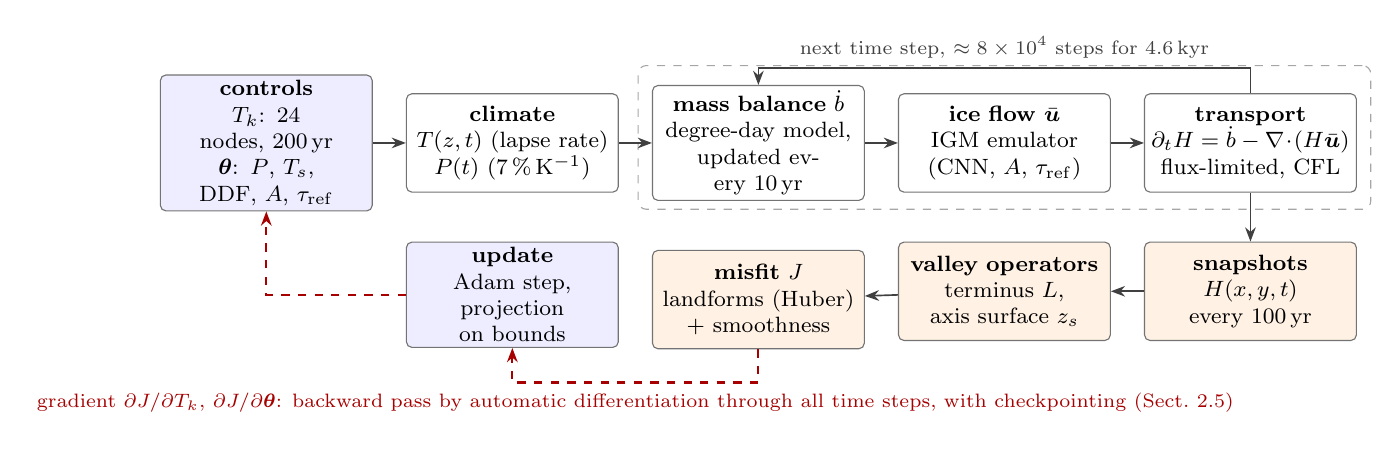
\begin{tikzpicture}[
  font=\footnotesize,
  box/.style={draw=black!55, rounded corners=2pt, align=center, minimum height=1.25cm, text width=2.55cm, fill=white, inner sep=2pt},
  ctl/.style={box, fill=blue!7},
  obsbox/.style={box, fill=orange!10},
  arr/.style={-{Stealth[length=1.8mm]}, semithick, black!75},
  gradarr/.style={-{Stealth[length=1.8mm]}, thick, red!65!black, dashed},
  node distance=0.62cm and 0.42cm]
\node[ctl] (T) {\textbf{controls}\\ $T_k$: 24 nodes, 200\,yr\\ $\boldsymbol\theta$: $P$, $T_s$, DDF, $A$, $\taur$};
\node[box, right=of T] (clim) {\textbf{climate}\\ $T(z,t)$ (lapse rate)\\ $P(t)$ (7\,\%\,\unit{K^{-1}})};
\node[box, right=of clim] (smb) {\textbf{mass balance} $\dot b$\\ degree-day model,\\ updated every 10\,yr};
\node[box, right=of smb] (flow) {\textbf{ice flow} $\ubar$\\ IGM emulator\\ (CNN, $A$, $\taur$)};
\node[box, right=of flow] (tr) {\textbf{transport}\\ $\partial_t H=\dot b-\nabla\!\cdot\!(H\ubar)$\\ flux-limited, CFL};
\node[obsbox, below=of tr] (snap) {\textbf{snapshots}\\ $H(x,y,t)$\\ every 100\,yr};
\node[obsbox, below=of flow] (ops) {\textbf{valley operators}\\ terminus $L$,\\ axis surface $z_s$};
\node[obsbox, below=of smb] (J) {\textbf{misfit} $J$\\ landforms (Huber)\\ + smoothness};
\node[ctl, below=of clim] (adam) {\textbf{update}\\ Adam step,\\ projection on bounds};
\draw[arr] (T) -- (clim);
\draw[arr] (clim) -- (smb);
\draw[arr] (smb) -- (flow);
\draw[arr] (flow) -- (tr);
\draw[arr] (tr.north) -- ++(0,0.32) -| node[pos=0.25, above, font=\scriptsize]{next time step, $\approx 8\times10^4$ steps for 4.6\,kyr} (smb.north);
\draw[arr] (tr) -- (snap);
\draw[arr] (snap) -- (ops);
\draw[arr] (ops) -- (J);
\draw[gradarr] (J.south) -- ++(0,-0.42) -| node[pos=0.25, below, font=\scriptsize, text=red!65!black, align=center]
  {gradient $\partial J/\partial T_k$, $\partial J/\partial\boldsymbol\theta$: backward pass by automatic differentiation through all time steps, with checkpointing (Sect.~2.5)} (adam.south);
\draw[gradarr] (adam.west) -| (T.south);
\begin{scope}[on background layer]
\node[draw=black!35, dashed, rounded corners=3pt, fit=(smb)(flow)(tr), inner sep=5pt, yshift=2pt] (loop) {};
\end{scope}
\end{tikzpicture}
\end{document}
